\documentclass[a4paper, top=10mm]{article}
%for writing from the top
\usepackage{fullpage}
%for math
\usepackage{amsmath}
\usepackage{mathrsfs}
\usepackage{amsthm}
%for images
\usepackage{graphicx}
%for color
\usepackage{xcolor}
%for title
\title{\textbf{\huge{Christmas Balls}}}
\author{Enigma n\textsuperscript{o}8}
\date{14\textsuperscript{th} December 2023}

\newtheorem*{hint}{Hint}

\addtolength{\voffset}{-2cm}
\addtolength{\textheight}{5cm}


\begin{document}
	\maketitle
	
	You are manufacturing magical Christmas decorations.
	All of them  are $n$-dimensional balls (hyper-balls, if you prefer), and they all have a radius of one.
	However, the decorations are magical, and may live in any dimension.
	You want to know what is the minimal and maximal volume of the decorations.
	
	\begin{center}
		
\includegraphics[width=0.3\linewidth]{08dimension1.png}	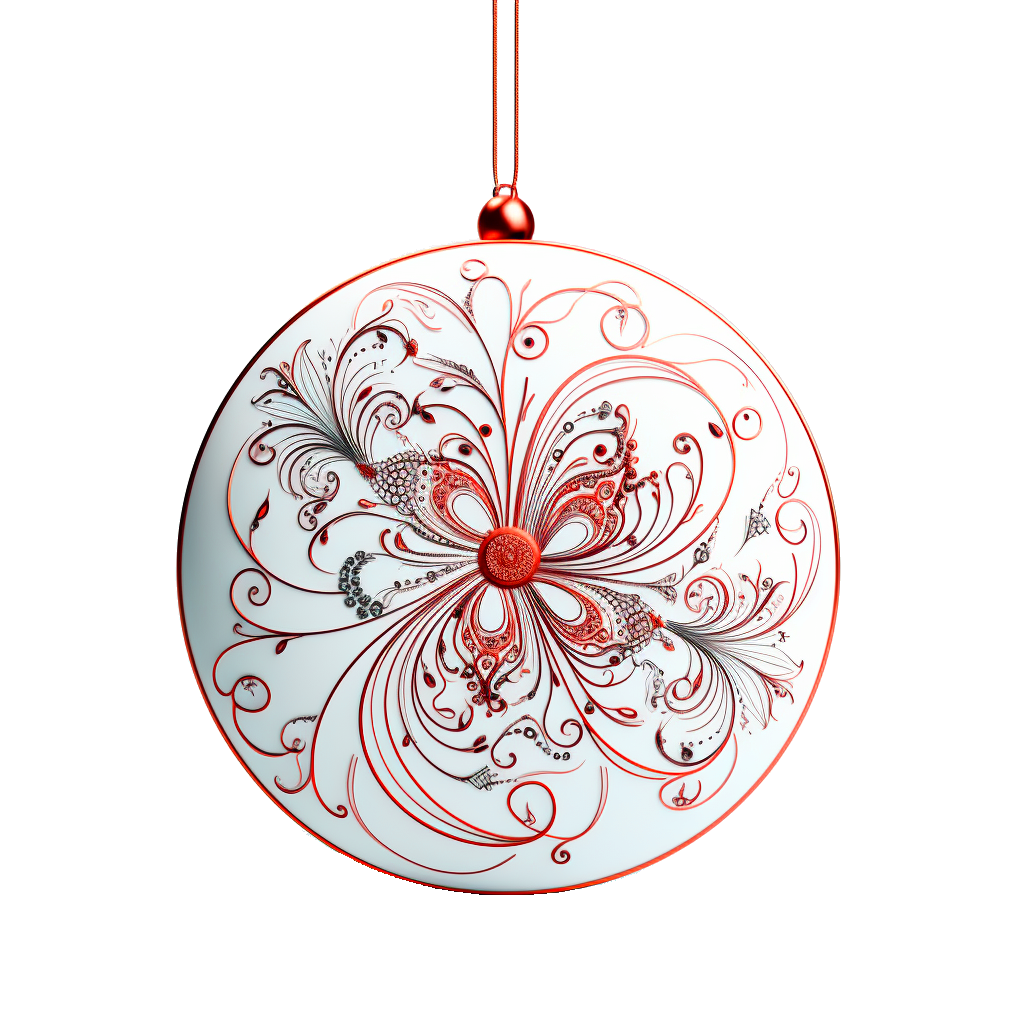
\includegraphics[width=0.3\linewidth]{08dimension2.png}		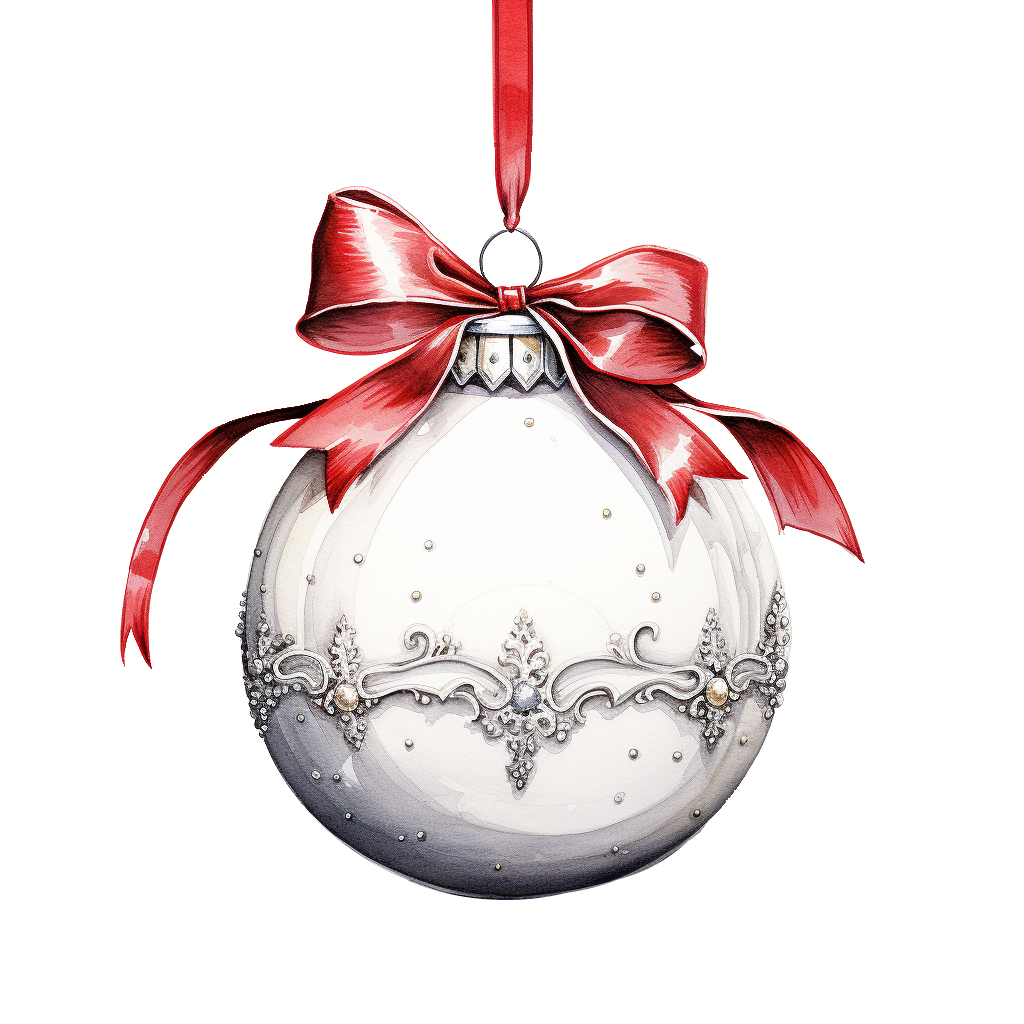
\includegraphics[width=0.3\linewidth]{08dimension3.png}
		
		Christmas decorations in 1,2 and 3 dimensions.
	\end{center}
	
	The volume of a $n$-dimensional ball of radius $R$ is given by: $\mathcal{V} = C_n R^n$.
	The constants $C_n$ follow the rule $C_n = \frac{2\pi}{n} \cdot C_{n-2}$.
	
	
\end{document}